% =====================================================================
% fig:families — full-width (figure*) schematic of the five morph
% families whose generation shortcuts are analyzed in the paper:
% MAD22 landmark-warping pipelines (FaceMorpher, OpenCV, WebMorph:
% landmark detection -> warp -> blend, differing in blend geometry /
% post-processing: halo ring, blur, JPEG) and GAN synthesis
% (MIPGAN-I, MIPGAN-II). Aggregations as in tab:mad22_results:
% LM2 = mean(OpenCV, WebMorph), M4 = mean(MIPGAN-I, MIPGAN-II).
% The same recipes were re-stamped on the five FRLL-Morphs families
% \`a la MAD22 (tab:frll_results).
% ---------------------------------------------------------------------
% Self-contained TikZ. No raster assets, no real faces: schematic icons
% only (see figures/teaser.tex header for the clearance note). Palette
% tzBlue/tzOrange/tzGray/tzDark/tzRed defined locally, teaser-consistent.
% Smallest text: \scriptsize. Uses scope+pic (NOT node-nested inline
% \tikz with pics -- that variant loops TeX indefinitely).
% ---------------------------------------------------------------------
% Intended placement (see commented OPTIONAL FIGURE INCLUDES block in
% main.tex, or move to method.tex): near the paragraph
% "Morph corpora and family reconstruction".
% =====================================================================
\begin{figure*}[t]
\centering
\resizebox{\textwidth}{!}{%
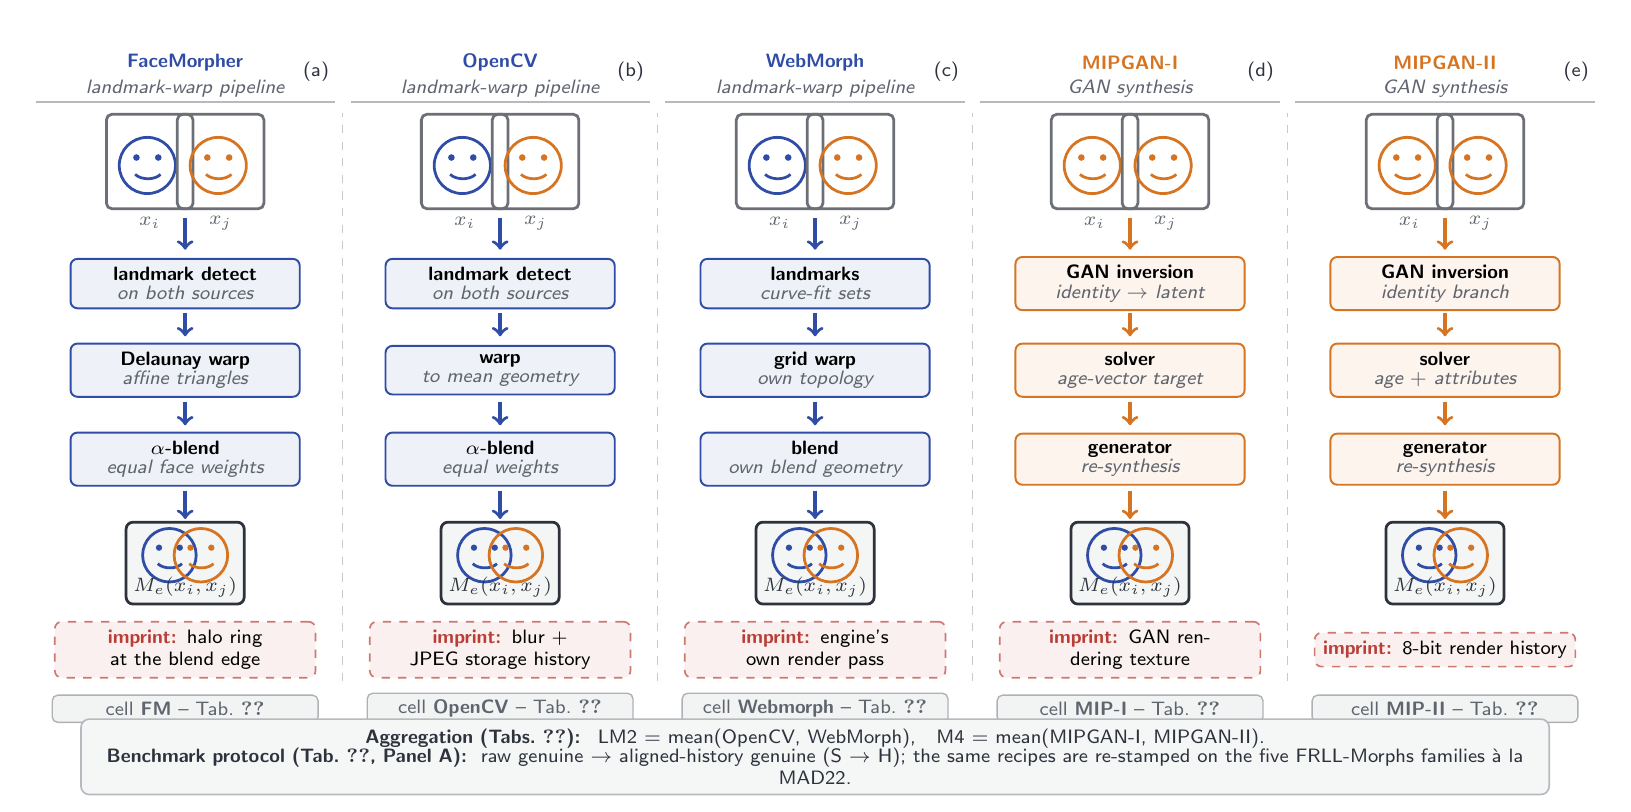
\begin{tikzpicture}[
  x=1cm,y=1cm,
  font=\sffamily,
  every node/.style={align=center, inner sep=1.5pt, outer sep=0pt},
  fline/.style={line width=1.0pt},
  hrule/.style={draw=tzGray!45, line width=0.6pt},
  vsep/.style={draw=tzGray!35, dashed, line width=0.6pt},
  flowlm/.style={->, tzBlue, line width=1.2pt},
  flowgan/.style={->, tzOrange, line width=1.2pt},
  lmchip/.style={draw=tzBlue, fill=tzBlue!8, rounded corners=2.5pt,
                 line width=0.7pt, text width=2.7cm,
                 font=\sffamily\scriptsize, inner sep=3pt},
  ganchip/.style={draw=tzOrange, fill=tzOrange!8, rounded corners=2.5pt,
                  line width=0.7pt, text width=2.7cm,
                  font=\sffamily\scriptsize, inner sep=3pt},
  imprint/.style={draw=tzRed!70, fill=tzRed!8, dashed, rounded corners=2.5pt,
                  line width=0.6pt, text width=3.1cm,
                  font=\sffamily\scriptsize, inner sep=3pt},
  bench/.style={draw=tzGray!50, fill=tzGray!8, rounded corners=2pt,
                line width=0.5pt, text width=3.2cm,
                font=\sffamily\scriptsize, inner sep=2.5pt, text=tzGray},
  pname/.style={font=\sffamily\bfseries\scriptsize},
  ptag/.style={font=\sffamily\scriptsize\itshape, text=tzGray},
  hint/.style={font=\sffamily\scriptsize, text=tzGray},
  stamp/.style={font=\sffamily\scriptsize, text=tzDark},
]
\useasboundingbox (0,0) rectangle (20,9.6);
\definecolor{tzBlue}{RGB}{47,76,166}
\definecolor{tzOrange}{RGB}{214,116,34}
\definecolor{tzGray}{RGB}{95,100,110}
\definecolor{tzDark}{RGB}{45,50,60}
\definecolor{tzRed}{RGB}{186,62,54}

\tikzset{
  % abstract, generic line-art face (identical to teaser's icon)
  picface/.pic={
    \draw[fline, pic actions] (0,0) circle (0.85);
    \fill[pic actions] (-0.33,0.24) circle (0.10);
    \fill[pic actions] (0.33,0.24) circle (0.10);
    \draw[fline, pic actions] (-0.37,-0.27) arc (215:325:0.47 and 0.31);
  },
}

% helper macros: sources pair, morph glyph ---------------------------
\newcommand{\famsources}[2]{% #1 = x center, #2 = flow color
  \begin{scope}[shift={(#1-0.45,7.9)}]
    \draw[fline, tzDark!70, rounded corners=2pt] (-0.55,-0.60) rectangle (0.55,0.60);
    \path (-0.03,-0.05) pic[scale=0.42, #2] {picface};
  \end{scope}
  \begin{scope}[shift={(#1+0.45,7.9)}]
    \draw[fline, tzDark!70, rounded corners=2pt] (-0.55,-0.60) rectangle (0.55,0.60);
    \path (-0.03,-0.05) pic[scale=0.42, tzOrange] {picface};
  \end{scope}
  \node[hint] at (#1-0.45,7.12) {$x_i$};
  \node[hint] at (#1+0.45,7.12) {$x_j$};
}
\newcommand{\fammorph}[1]{% #1 = x center; two contributors + frame
  \begin{scope}[shift={(#1,2.80)}]
    \draw[fline, tzDark, rounded corners=2.5pt, fill=tzDark!5]
      (-0.75,-0.52) rectangle (0.75,0.52);
    \path (-0.20,0.10) pic[scale=0.40, tzBlue] {picface};
    \path (0.20,0.10) pic[scale=0.40, tzOrange] {picface};
    \node[stamp] at (0,-0.30) {\scriptsize$M_e(x_i,x_j)$};
  \end{scope}
}

% ===================== PANEL (a): FaceMorpher ========================
\def\famx{2}
\node[pname, text=tzBlue] at (\famx,9.15) {FaceMorpher};
\node[ptag] at (\famx,8.82) {landmark-warp pipeline};
\draw[hrule] (\famx-1.9,8.66) -- (\famx+1.9,8.66);
\node[stamp, anchor=north east] at (\famx+1.88,9.22) {\scriptsize(a)};
\famsources{\famx}{tzBlue}
\draw[flowlm] (\famx,7.18) -- (\famx,6.78);
\node[lmchip] at (\famx,6.35) {\textbf{landmark detect}\\[-1pt]{\scriptsize\itshape\textcolor{tzGray}{on both sources}}};
\draw[flowlm] (\famx,5.98) -- (\famx,5.68);
\node[lmchip] at (\famx,5.25) {\textbf{Delaunay warp}\\[-1pt]{\scriptsize\itshape\textcolor{tzGray}{affine triangles}}};
\draw[flowlm] (\famx,4.85) -- (\famx,4.55);
\node[lmchip] at (\famx,4.12) {\textbf{$\alpha$-blend}\\[-1pt]{\scriptsize\itshape\textcolor{tzGray}{equal face weights}}};
\draw[flowlm] (\famx,3.72) -- (\famx,3.36);
\fammorph{\famx}
\node[imprint] at (\famx,1.70) {\textcolor{tzRed}{\textbf{imprint:}} halo ring at the blend edge};
\node[bench] at (\famx,0.95) {cell \textbf{FM} -- Tab.~\ref{tab:mad22_results}};

% ===================== PANEL (b): OpenCV =============================
\def\famx{6}
\node[pname, text=tzBlue] at (\famx,9.15) {OpenCV};
\node[ptag] at (\famx,8.82) {landmark-warp pipeline};
\draw[hrule] (\famx-1.9,8.66) -- (\famx+1.9,8.66);
\node[stamp, anchor=north east] at (\famx+1.88,9.22) {\scriptsize(b)};
\famsources{\famx}{tzBlue}
\draw[flowlm] (\famx,7.18) -- (\famx,6.78);
\node[lmchip] at (\famx,6.35) {\textbf{landmark detect}\\[-1pt]{\scriptsize\itshape\textcolor{tzGray}{on both sources}}};
\draw[flowlm] (\famx,5.98) -- (\famx,5.68);
\node[lmchip] at (\famx,5.25) {\textbf{warp}\\[-1pt]{\scriptsize\itshape\textcolor{tzGray}{to mean geometry}}};
\draw[flowlm] (\famx,4.85) -- (\famx,4.55);
\node[lmchip] at (\famx,4.12) {\textbf{$\alpha$-blend}\\[-1pt]{\scriptsize\itshape\textcolor{tzGray}{equal weights}}};
\draw[flowlm] (\famx,3.72) -- (\famx,3.36);
\fammorph{\famx}
\node[imprint] at (\famx,1.70) {\textcolor{tzRed}{\textbf{imprint:}} blur + JPEG storage history};
\node[bench] at (\famx,0.95) {cell \textbf{OpenCV} -- Tab.~\ref{tab:mad22_results}};

% ===================== PANEL (c): WebMorph ===========================
\def\famx{10}
\node[pname, text=tzBlue] at (\famx,9.15) {WebMorph};
\node[ptag] at (\famx,8.82) {landmark-warp pipeline};
\draw[hrule] (\famx-1.9,8.66) -- (\famx+1.9,8.66);
\node[stamp, anchor=north east] at (\famx+1.88,9.22) {\scriptsize(c)};
\famsources{\famx}{tzBlue}
\draw[flowlm] (\famx,7.18) -- (\famx,6.78);
\node[lmchip] at (\famx,6.35) {\textbf{landmarks}\\[-1pt]{\scriptsize\itshape\textcolor{tzGray}{curve-fit sets}}};
\draw[flowlm] (\famx,5.98) -- (\famx,5.68);
\node[lmchip] at (\famx,5.25) {\textbf{grid warp}\\[-1pt]{\scriptsize\itshape\textcolor{tzGray}{own topology}}};
\draw[flowlm] (\famx,4.85) -- (\famx,4.55);
\node[lmchip] at (\famx,4.12) {\textbf{blend}\\[-1pt]{\scriptsize\itshape\textcolor{tzGray}{own blend geometry}}};
\draw[flowlm] (\famx,3.72) -- (\famx,3.36);
\fammorph{\famx}
\node[imprint] at (\famx,1.70) {\textcolor{tzRed}{\textbf{imprint:}} engine's own render pass};
\node[bench] at (\famx,0.95) {cell \textbf{Webmorph} -- Tab.~\ref{tab:mad22_results}};

% ===================== PANEL (d): MIPGAN-I ===========================
\def\famx{14}
\node[pname, text=tzOrange] at (\famx,9.15) {MIPGAN-I};
\node[ptag] at (\famx,8.82) {GAN synthesis};
\draw[hrule] (\famx-1.9,8.66) -- (\famx+1.9,8.66);
\node[stamp, anchor=north east] at (\famx+1.88,9.22) {\scriptsize(d)};
\famsources{\famx}{tzOrange}
\draw[flowgan] (\famx,7.18) -- (\famx,6.78);
\node[ganchip] at (\famx,6.35) {\textbf{GAN inversion}\\[-1pt]{\scriptsize\itshape\textcolor{tzGray}{identity $\to$ latent}}};
\draw[flowgan] (\famx,5.98) -- (\famx,5.68);
\node[ganchip] at (\famx,5.25) {\textbf{solver}\\[-1pt]{\scriptsize\itshape\textcolor{tzGray}{age-vector target}}};
\draw[flowgan] (\famx,4.85) -- (\famx,4.55);
\node[ganchip] at (\famx,4.12) {\textbf{generator}\\[-1pt]{\scriptsize\itshape\textcolor{tzGray}{re-synthesis}}};
\draw[flowgan] (\famx,3.72) -- (\famx,3.36);
\fammorph{\famx}
\node[imprint] at (\famx,1.70) {\textcolor{tzRed}{\textbf{imprint:}} GAN rendering texture};
\node[bench] at (\famx,0.95) {cell \textbf{MIP-I} -- Tab.~\ref{tab:mad22_results}};

% ===================== PANEL (e): MIPGAN-II ==========================
\def\famx{18}
\node[pname, text=tzOrange] at (\famx,9.15) {MIPGAN-II};
\node[ptag] at (\famx,8.82) {GAN synthesis};
\draw[hrule] (\famx-1.9,8.66) -- (\famx+1.9,8.66);
\node[stamp, anchor=north east] at (\famx+1.88,9.22) {\scriptsize(e)};
\famsources{\famx}{tzOrange}
\draw[flowgan] (\famx,7.18) -- (\famx,6.78);
\node[ganchip] at (\famx,6.35) {\textbf{GAN inversion}\\[-1pt]{\scriptsize\itshape\textcolor{tzGray}{identity branch}}};
\draw[flowgan] (\famx,5.98) -- (\famx,5.68);
\node[ganchip] at (\famx,5.25) {\textbf{solver}\\[-1pt]{\scriptsize\itshape\textcolor{tzGray}{age $+$ attributes}}};
\draw[flowgan] (\famx,4.85) -- (\famx,4.55);
\node[ganchip] at (\famx,4.12) {\textbf{generator}\\[-1pt]{\scriptsize\itshape\textcolor{tzGray}{re-synthesis}}};
\draw[flowgan] (\famx,3.72) -- (\famx,3.36);
\fammorph{\famx}
\node[imprint] at (\famx,1.70) {\textcolor{tzRed}{\textbf{imprint:}} 8-bit render history};
\node[bench] at (\famx,0.95) {cell \textbf{MIP-II} -- Tab.~\ref{tab:mad22_results}};

% ------------------------------------------------- panel separations
\foreach \sx in {4,8,12,16}{\draw[vsep] (\sx,1.30) -- (\sx,8.52);}

% ------------------------------------------------ bottom summary strip
\node[draw=tzGray!45, fill=tzGray!6, rounded corners=3pt, line width=0.6pt,
      text width=18.4cm, font=\sffamily\scriptsize, inner sep=3.5pt,
      text=tzDark] at (10,0.34)
 {{\textbf{Aggregation (Tabs.~\ref{tab:mad22_results}):\ } LM2~$=$~mean(OpenCV,~WebMorph),\quad M4~$=$~mean(MIPGAN-I,~MIPGAN-II).}\\[-1pt]
  {\textbf{Benchmark protocol (Tab.~\ref{tab:mad22_results}, Panel~A):\ } raw genuine $\rightarrow$ aligned-history genuine (S~$\rightarrow$~H); the same recipes are re-stamped on the five FRLL-Morphs families \`a la MAD22.}};

\end{tikzpicture}}%
\captionsetup{hypcap=false}
\caption{The five morph families covered by the shortcut analysis (schematic; no real-face imagery).
\textbf{Blue:} landmark-warping pipelines -- landmark detection, geometric warp, blending -- that share the construction but differ in blend geometry and post-processing (FaceMorpher's halo ring, OpenCV's blur/JPEG storage history, WebMorph's own warp and blend field).
\textbf{Orange:} GAN synthesis in two variants (MIPGAN-I, MIPGAN-II).
Each panel annotates the processing trace most likely to \emph{imprint} -- the imprint a shortcut detector can latch onto without seeing two identities.
All families are benchmarked in Table~\ref{tab:mad22_results} under the raw-to-aligned-history genuine protocol (S~$\to$~H, Panel~A); aggregations average OpenCV$+$WebMorph into LM2 and MIPGAN-I$/$II into M4.
The same recipes were re-applied to rebuild the five FRLL-Morphs families \`a la MAD22 (Table~\ref{tab:frll_results}).}
\label{fig:families}
\end{figure*}
